\subsubsection{Electrocardiogram (ECG) data}
\label{subsubsec:results_ecg_1}


As previously stated, the ECG analysis is based on two variables: the heartrate (BPM – beats per minute) and heartrate variance (SDNN – standard deviation of NN intervals). 

After the experiment, the ECG signal processing is organized in the following steps: 

\begin{itemize}
    \item Filtering and removal of outliers, since the participants moved during the whole experience, the sensors captured also a significant amount of noise. 
    \item Normalization between -1 and 1;
    \item Peak detection and evaluation – if the results were not of good quality, peak detection method’s parameters were adjusted to improve it; 
    \item Calculation of BPM using Kubius HRV Standard;
    \item Calculation of SDNN using Kubius HRV Standard.
\end{itemize}

At the beginning of each experiment, a baseline was collected to establish a comparison between the relaxed state of the participant and the scenes’ induced state. However, the results were not consistent. It was expected that the heartrate would increase during the experiment, comparing to the baseline, because the participants were at rest. But for most of the participants, it actually decreased, indicating a systematic problem may have occurred. Due to this fact, the analysis is based only on absolute values.

\paragraph{Analysis of the heartbeat frequency (BPM)}\mbox{}\\

Table \ref{tab:bpm_table_blind}  presents the heart rate of each blind participant for each guidance method. It is possible to observe that there is no systematic difference among the methods. Also, there are significant differences among the participants, which some of them presenting values significantly lower than others.


\begin{table}[!htb]
\centering
\caption{Average BPM felled by the blinded participants [BPM].}
\label{tab:bpm_table_blind}
\begin{tabular}{llrrrrr}
\toprule
     &        &   Base &  Audio & \begin{tabular}[c]{@{}l@{}}Haptic\\ Belt\end{tabular} & \begin{tabular}[c]{@{}l@{}}Virtual\\ Cane\end{tabular} & Mixture \\
Participant & Round &        &        &                                                       &                                                        &         \\
\midrule
001C & First &  75.75 &  60.71 &                                                 71.17 &                                                  59.07 &   68.24 \\
     & Return &  71.05 &  58.61 &                                                 66.22 &                                                  64.20 &   70.76 \\
002C & First &  48.69 &  38.67 &                                                 48.74 &                                                  46.89 &   52.23 \\
     & Return &  52.46 &  47.58 &                                                 58.97 &                                                  56.75 &   58.25 \\
003C & First &  68.37 &  69.89 &                                                 70.95 &                                                  69.41 &   66.94 \\
     & Return &  67.34 &  67.44 &                                                 69.68 &                                                  68.82 &   67.37 \\
004C & First &  75.09 &  73.55 &                                                 73.70 &                                                  71.94 &   74.03 \\
     & Return &  74.74 &  74.79 &                                                 74.02 &                                                  72.69 &   67.34 \\
\bottomrule
\end{tabular}
\end{table}



Figure \ref{fig:barplot_ecg_bpm_5_scene_blind} presents the mean heart rate. It shows a slight increase in the heartrate between the rounds, with the exception of the ‘base’ method, indicating that the participants felt the ‘return’ round more demandful.

\begin{figure}[!htb]
    \centering
    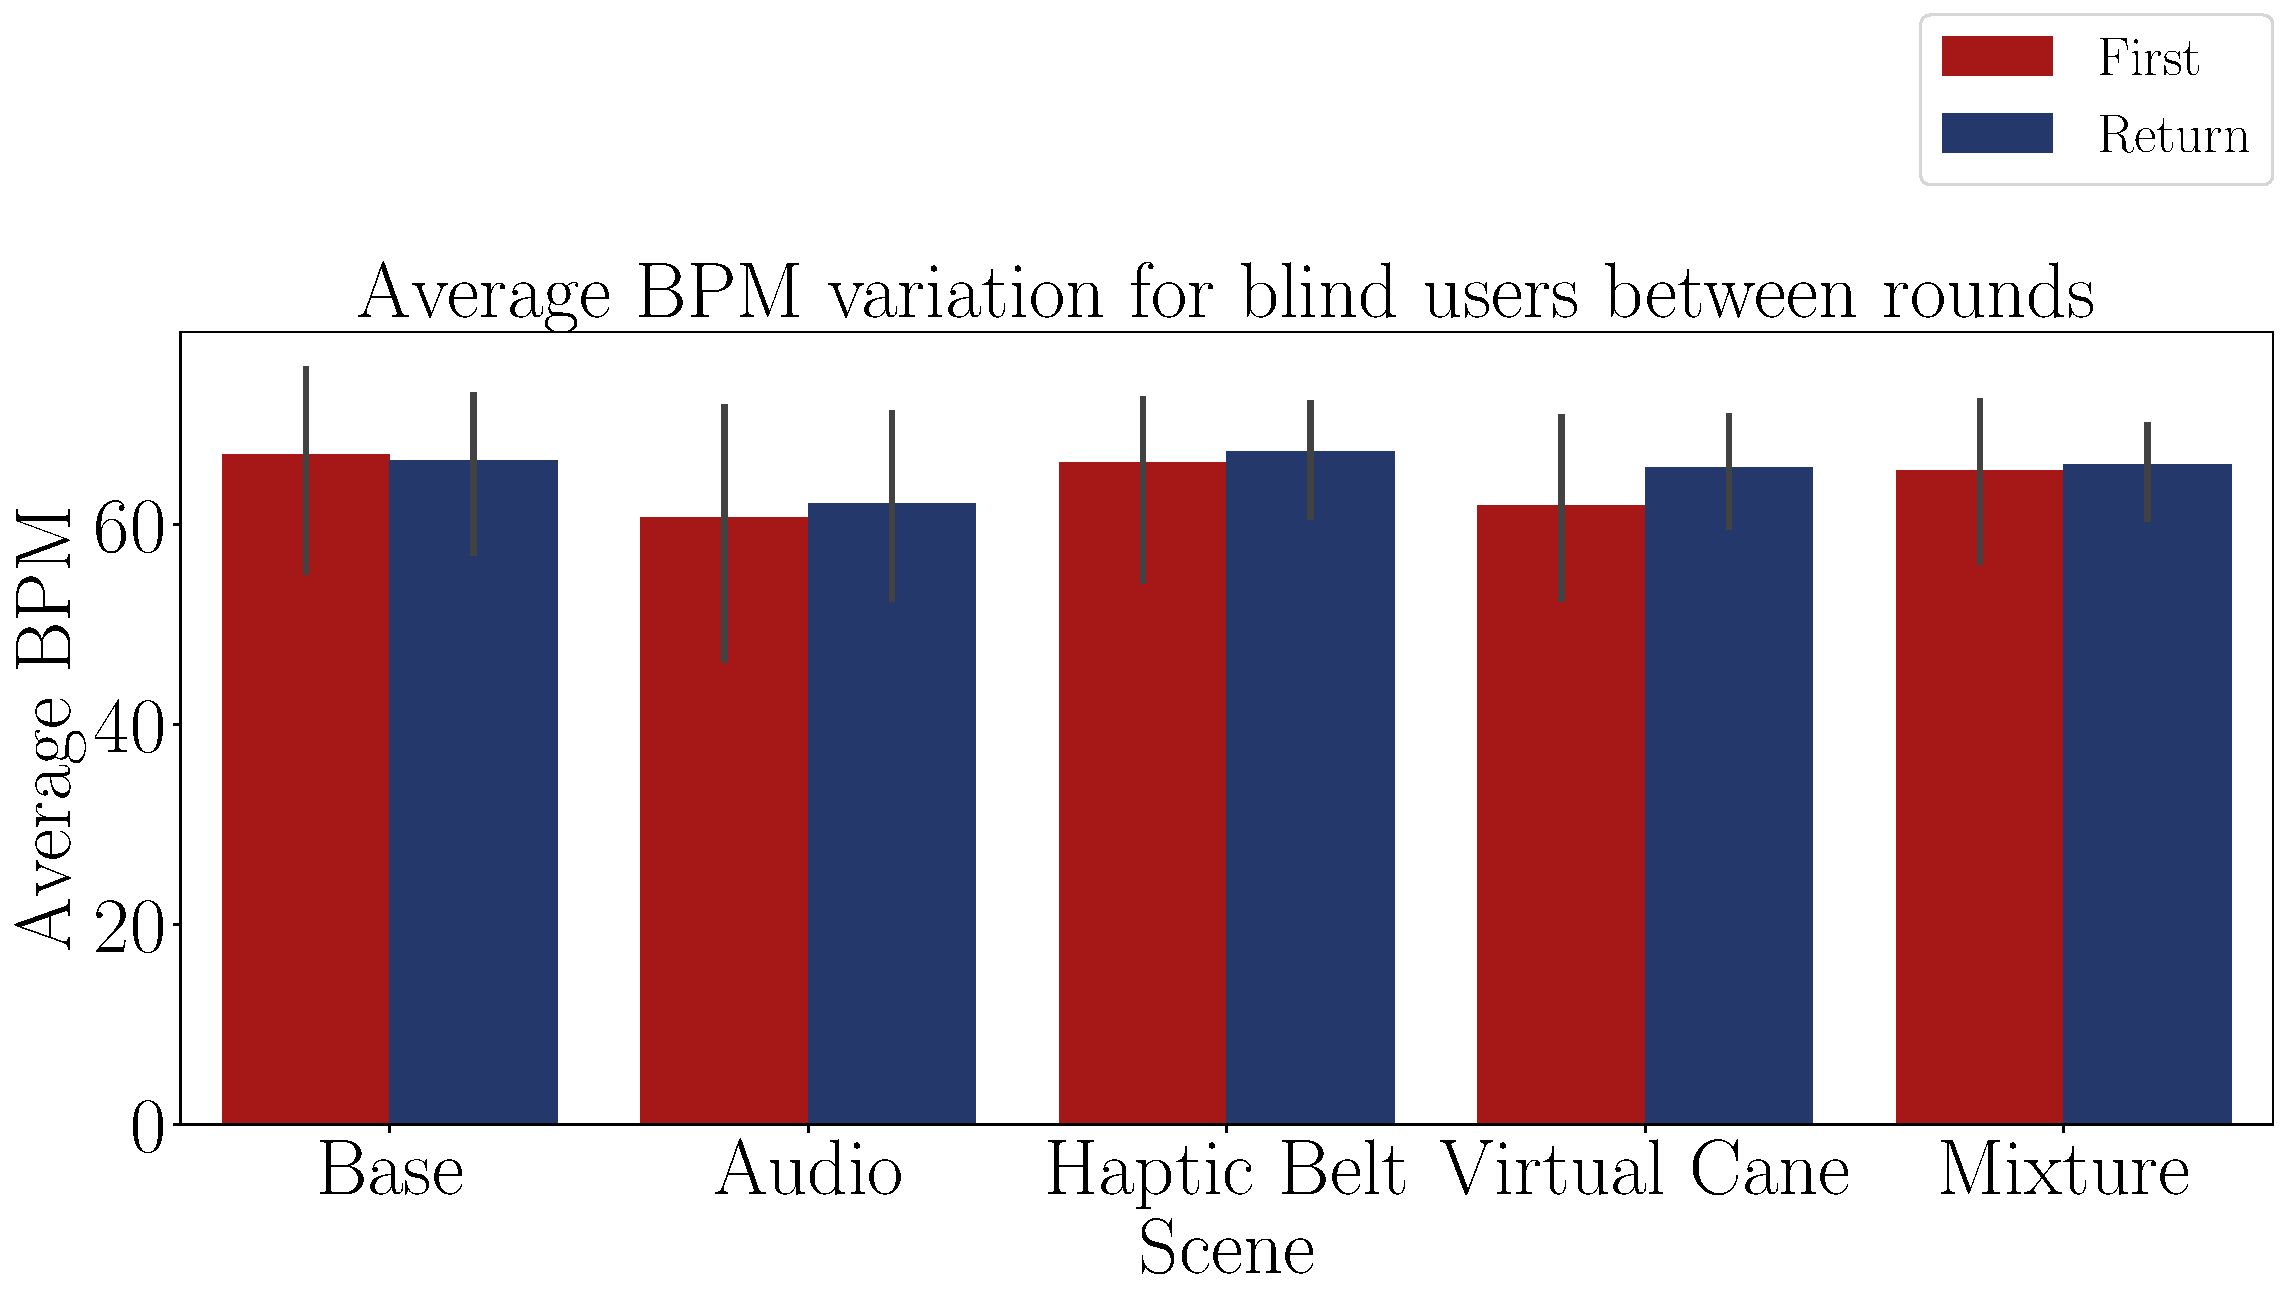
\includegraphics[width = 0.8\linewidth]{Resultados/ECG/Figuras/pdf/barplot_ecg_bpm_5_scene_blind.pdf}
    \caption{Barplot of the average BPM of the blind participants on each method.}
    \label{fig:barplot_ecg_bpm_5_scene_blind}
\end{figure}

%The Table \ref{tab:bpm_average_group_blind} show the average heartbeat frequency variation between the rounds of each group. As it was shown in the Figure \ref{fig:barplot_ecg_bpm_5_scene_blind}, only the "Base" method has a negative average variaton between the rounds. It is also posible to see that the Virtual Cane variation was the highest, hence it was also the highest mental workload.
% 
%
\begin{table}[!htb]
\centering
\caption{ECG average BPM  for each method of the blind participants.}
\label{tab:bpm_average_group_blind}
\begin{tabular}{lrrrrr}
\toprule
{} &   Base & Audio & Haptic Belt & Virtual Cane & Mixture \\
Visual Condition &        &       &             &              &         \\
\midrule
Blind            &  -0.58 &  1.40 &        1.09 &         3.79 &    0.57 \\
\bottomrule
\end{tabular}
\end{table}



Figures \ref{fig:boxplot_ecg_bpm_blind_scene} and \ref{fig:boxplot_ecg_bpm_blind_rounds} brings the corresponding boxplot, grouped by method and round. In both cases, it is not possible to observe significant differences among the methods or rounds.

\begin{figure}[!htb]
    \centering
    \begin{minipage}{0.45\textwidth}
        \centering
        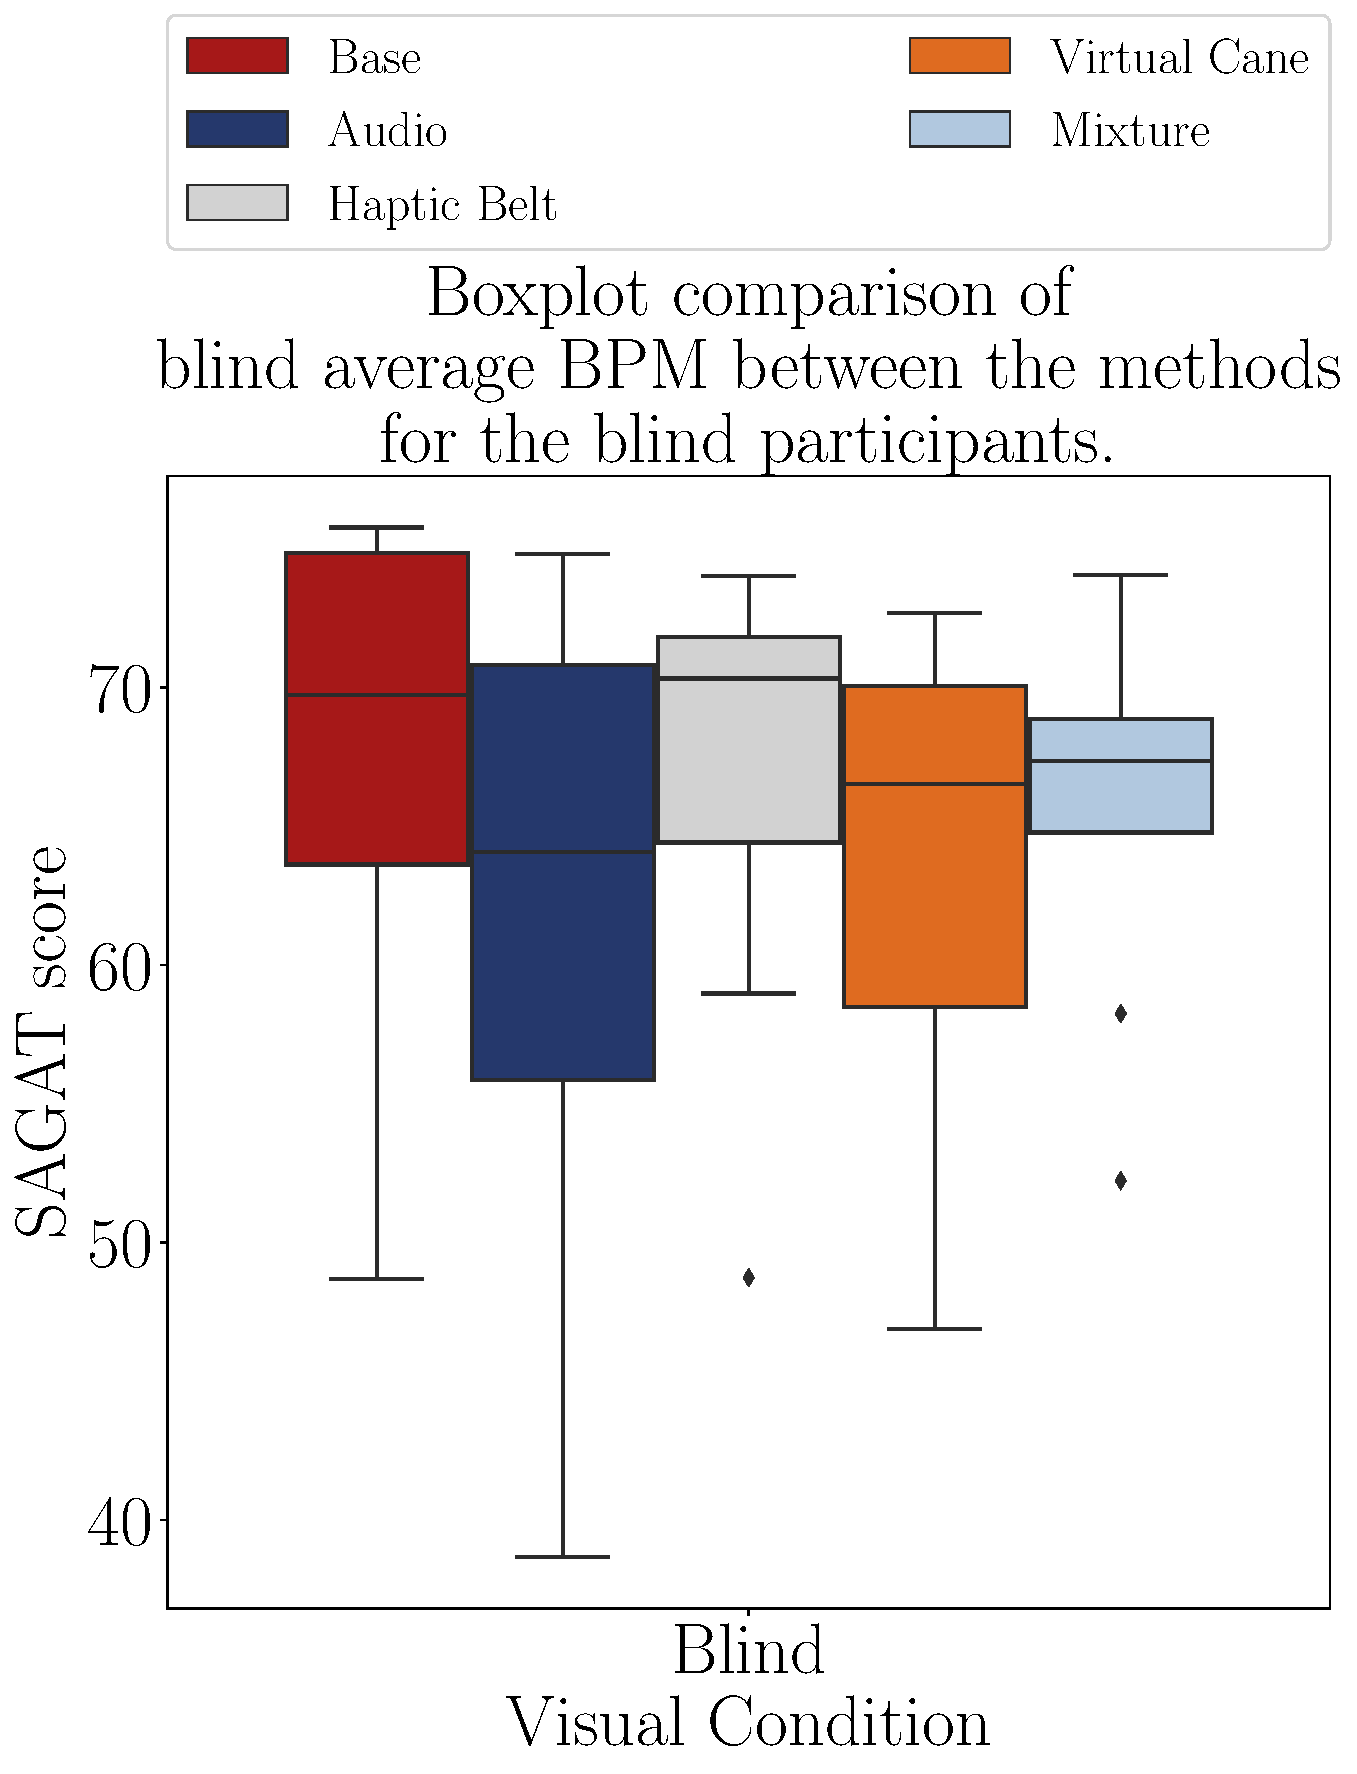
\includegraphics[width = 0.8\linewidth]{Resultados/ECG/Figuras/pdf/boxplot_ecg_bpm_blind_scene.pdf}
        \caption{Boxplot of the BPM of the blind participants grouped by method.}
        \label{fig:boxplot_ecg_bpm_blind_scene}
    \end{minipage}
    \begin{minipage}{0.075\textwidth}
        \hfill
    \end{minipage}
    \begin{minipage}{0.45\textwidth}
        \centering
        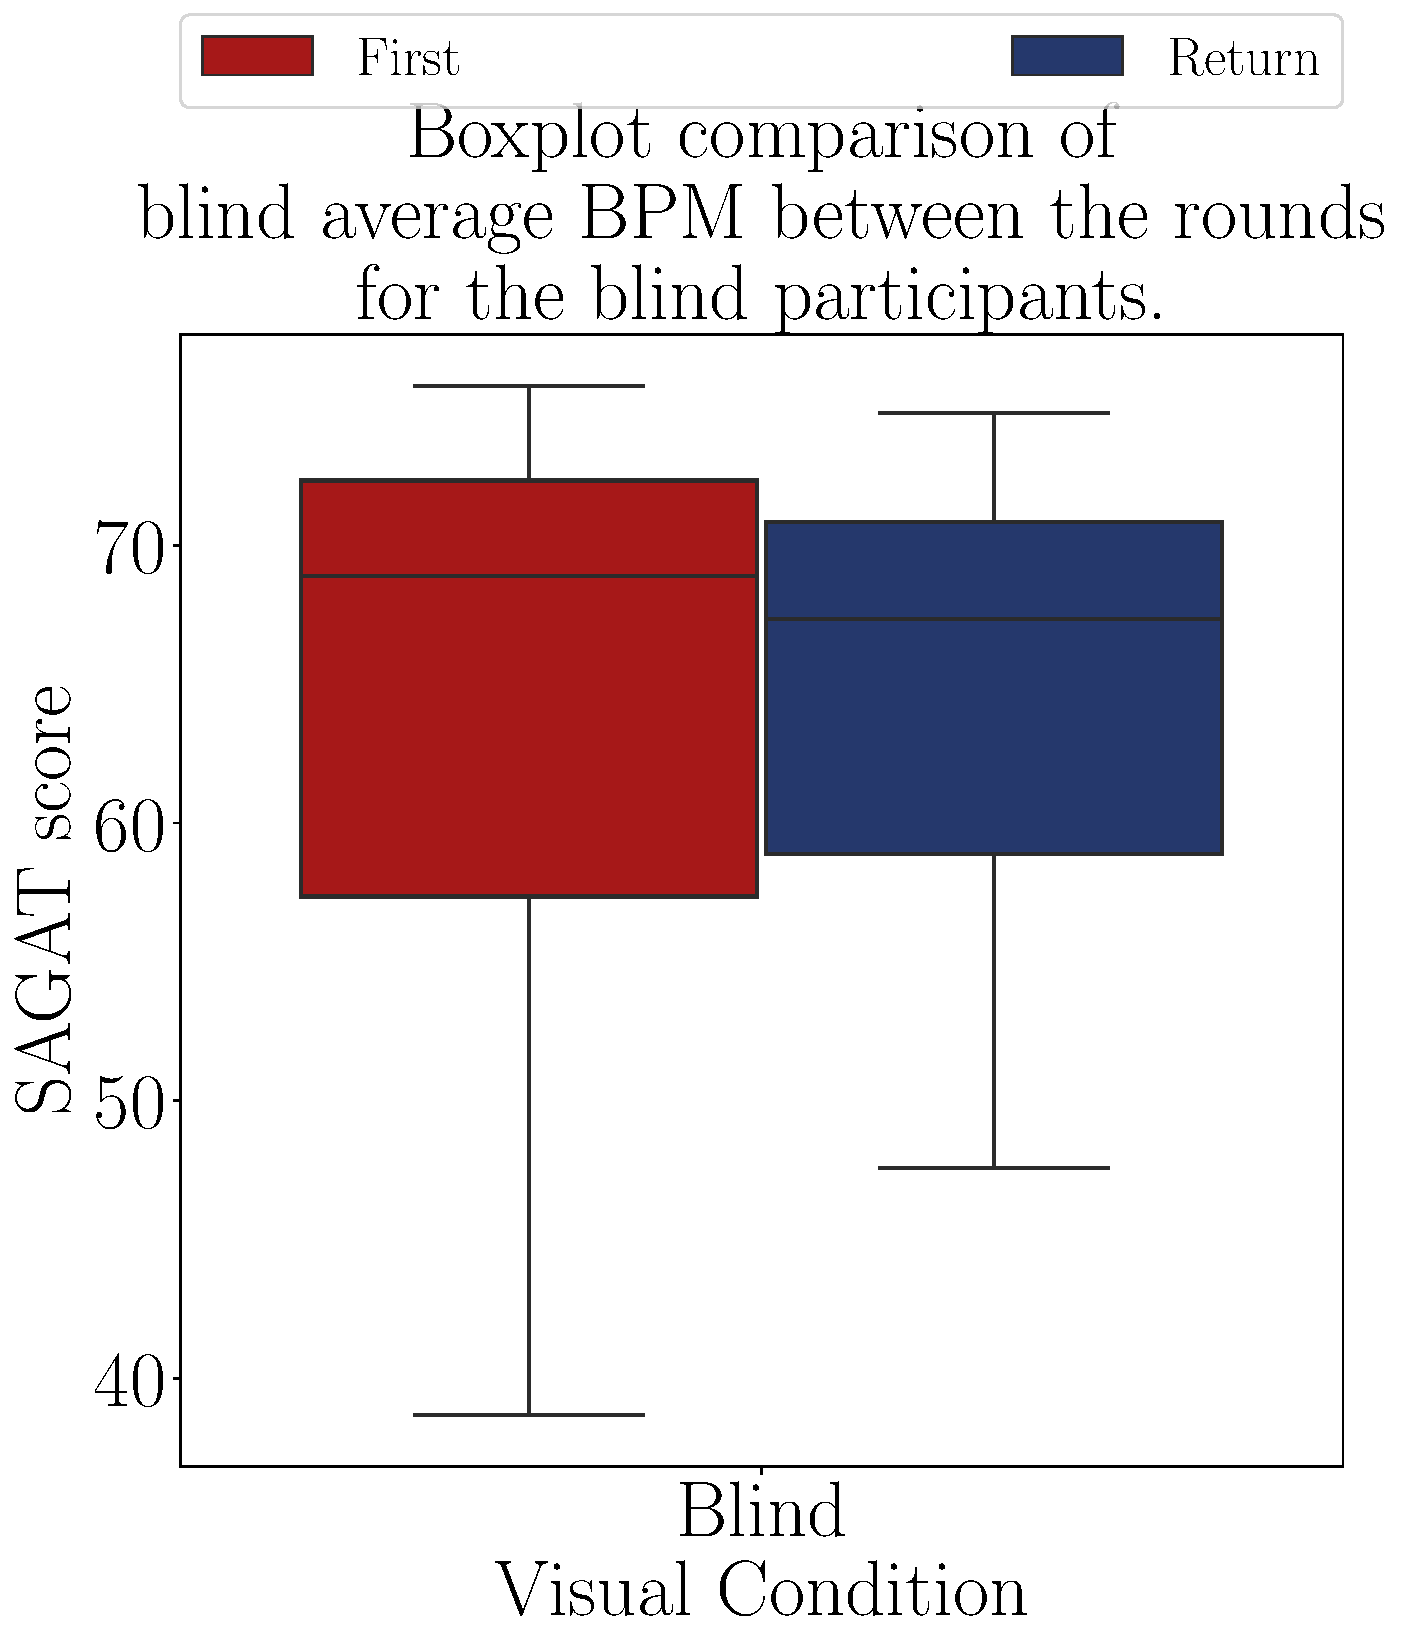
\includegraphics[width = 0.8\linewidth]{Resultados/ECG/Figuras/pdf/boxplot_ecg_bpm_blind_rounds.pdf}
        \caption{Boxplot of the BPM of the blind participants grouped by round.}
        \label{fig:boxplot_ecg_bpm_blind_rounds}
    \end{minipage}
\end{figure}

Figures \ref{fig:qqplot_bpm_two_way_blind} and \ref{fig:residplot_bpm_two_way_blind} bring the QQ Plot and residual distribution. Particularly, the last one shows that the participant does not have similar variance, which may jeopardize the results of ANOVA. Considering this limitation, Table \ref{tab:bpm_table_blind} brings the p-value obtained by ANOVA, which confirmed the previous analysis, as it does not indicate a significant influence of either the guidance method or the round in the participants heartrate. 

\begin{figure}[!htb]
    \centering
    \begin{minipage}{0.45\textwidth}
        \centering
        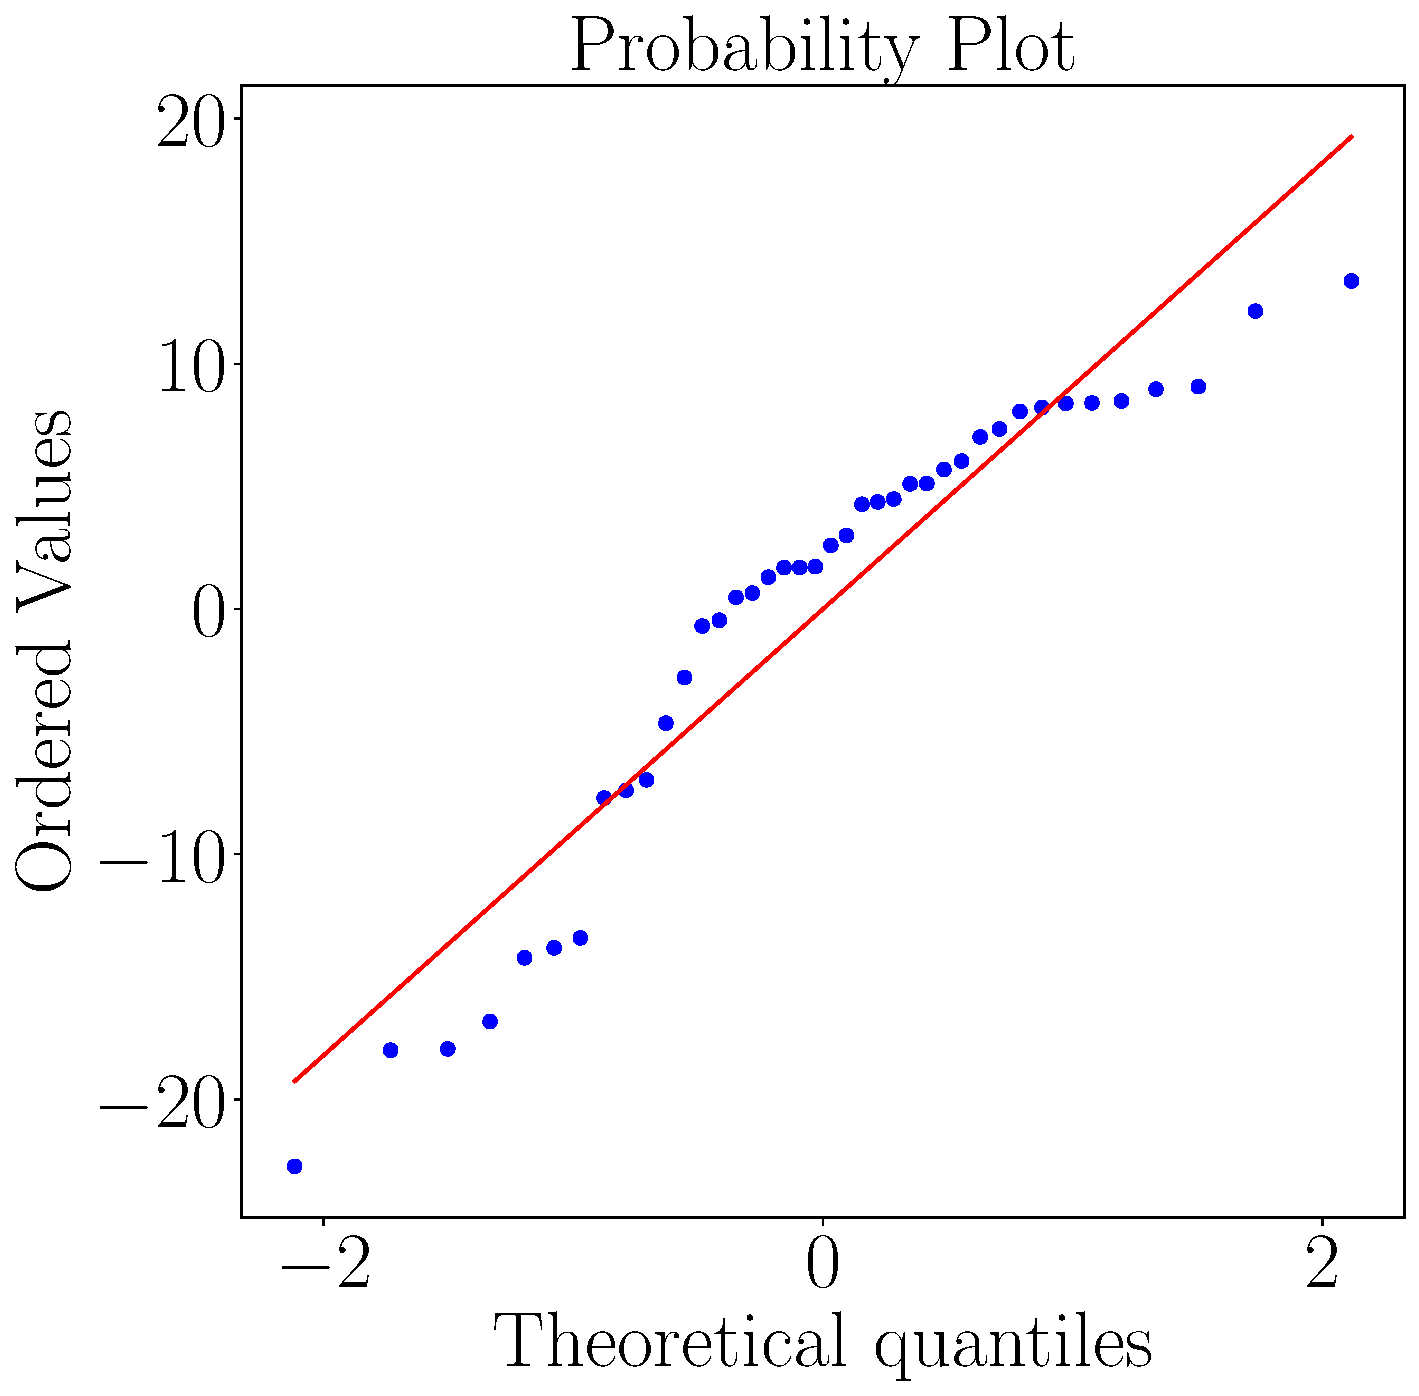
\includegraphics[width = 0.8\linewidth]{Resultados/ECG/Figuras/pdf/qqplot_bpm_two_way_blind.pdf}
        \caption{QQ plot of the BPM of the blind participants on each method.}
        \label{fig:qqplot_bpm_two_way_blind}
    \end{minipage}
    \begin{minipage}{0.075\textwidth}
        \hfill
    \end{minipage}
    \begin{minipage}{0.45\textwidth}
        \centering
        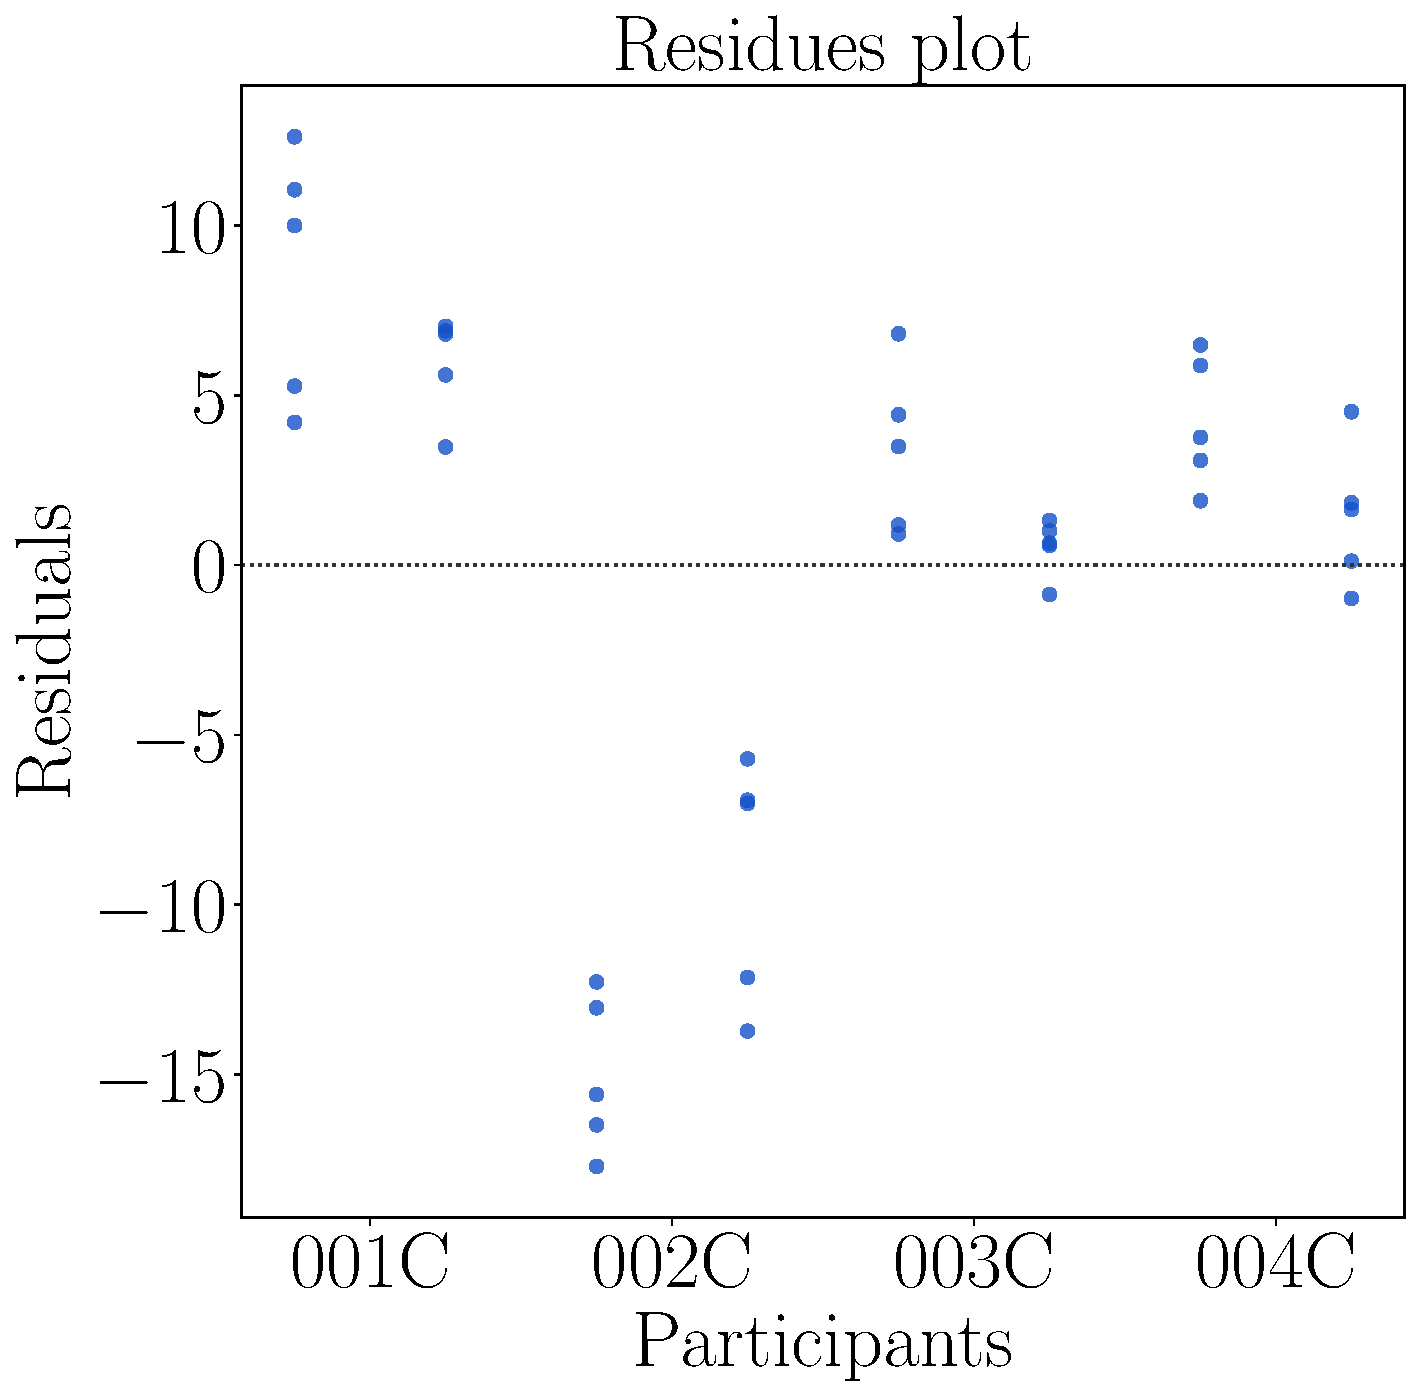
\includegraphics[width = 0.8\linewidth]{Resultados/ECG/Figuras/pdf/residplot_bpm_two_way_blind.pdf}
        \caption{Residual plot of the BPM score the blind participants on each method.}
        \label{fig:residplot_bpm_two_way_blind}
    \end{minipage}
\end{figure}


\begin{table}[!htb]
\centering
\caption{Anova p-value for the BPM on each method for blinded users.}
\label{tab:blocanova_bpm_two_way_blind}
\begin{tabular}{lrrrrr}
\toprule
               Source &  Squared sum &  DOF & Squared average &      F & \begin{tabular}[c]{@{}l@{}}P-Value \\ $(F_{0} > F)$\end{tabular} \\
\midrule
Participants (Blocks) &     2807.274 &    3 &         935.758 & 49.361 &                                                                  \\
         \    Methods &      164.045 &    4 &          41.011 &  2.163 &                                                            0.100 \\
          \    Rounds &       15.693 &    1 &          15.693 &  0.828 &                                                            0.371 \\
     \    Interaction &       20.606 &    4 &           5.152 &  0.272 &                                                            0.894 \\
   Experimental Error &      511.853 &   27 &          18.958 &        &                                                                  \\
                Total &     3519.471 &   39 &                 &        &                                                                  \\
\bottomrule
\end{tabular}
\end{table}



%
\begin{table}[!htb]
\centering
\caption{Cross validation p-value for the average BPM on each method for blinded users.}
\label{tab:lsd_bpm_two_way}
\begin{tabular}{rclr}
\toprule
      \multicolumn{3}{c}{Method} &                                           Analysis \\
\midrule
              Base & $X$ & Audio &               $H_1 : \mu_{Base} \ne \mu_{Audio}**$ \\
        Base & $X$ & Haptic Belt &             $H_0 : \mu_{Base} = \mu_{Haptic Belt}$ \\
       Base & $X$ & Virtual Cane &        $H_1 : \mu_{Base} \ne \mu_{Virtual Cane}**$ \\
            Base & $X$ & Mixture &             $H_1 : \mu_{Base} \ne \mu_{Mixture}**$ \\
       Audio & $X$ & Haptic Belt &        $H_1 : \mu_{Audio} \ne \mu_{Haptic Belt}**$ \\
      Audio & $X$ & Virtual Cane &       $H_1 : \mu_{Audio} \ne \mu_{Virtual Cane}**$ \\
           Audio & $X$ & Mixture &            $H_1 : \mu_{Audio} \ne \mu_{Mixture}**$ \\
Haptic Belt & $X$ & Virtual Cane & $H_1 : \mu_{Haptic Belt} \ne \mu_{Virtual Cane}**$ \\
     Haptic Belt & $X$ & Mixture &      $H_1 : \mu_{Haptic Belt} \ne \mu_{Mixture}**$ \\
    Virtual Cane & $X$ & Mixture &     $H_1 : \mu_{Virtual Cane} \ne \mu_{Mixture}**$ \\
\bottomrule
\end{tabular}
\end{table}



%The Table \ref{tab:lsd_bpm_two_way} presents the conclusion of a pairwise Fisher LSD test of the blind heart rate frequency variation between all the guidance methods. The results show that the only the "Base" and "Haptic belt" have simila reaction.

\FloatBarrier

%%%%%%%%%%%%%%%%%%%%%%%%%%%%%%%%%%%%%%%%%%%%%%%%%%%%%%%%%%%%%%%%%%%%%%%%%%%%
%%%%%%%%%%%%%%%%%%%%%%%%%%%%%%%%%%%%%%%%%%%%%%%%%%%%%%%%%%%%%%%%%%%%%%%%%%%%
%%%%%%%%%%%%%%%%%%%%%%%%%%%%%%%%%%%%%%%%%%%%%%%%%%%%%%%%%%%%%%%%%%%%%%%%%%%%
%%%%%%%%%%%%%%%%%%%%%%%%%%%%%%%%%%%%%%%%%%%%%%%%%%%%%%%%%%%%%%%%%%%%%%%%%%%%
%
%
\paragraph{Analysis of the heartbeat variance (SDNN)}\mbox{}\\
%
Table \ref{tab:sdnn_table_blind} brings the value of the second variable extracted from the ECG: SDNN, the standard deviation of the interbeat interval. Similar to what is observed for the BPM, it is not possible do draw a pattern from this data. Different participant had increase or decrease their heartrate, with different methods.


\begin{table}[!htb]
\centering
\caption{Average SDNN of the blind participants during the each round and method [ms].}
\label{tab:sdnn_table_blind}
\begin{tabular}{llrrrrr}
\toprule
     &        &    Base &   Audio &  \begin{tabular}[c]{@{}l@{}}Haptic\\ Belt\end{tabular} &  \begin{tabular}[c]{@{}l@{}}Virtual\\ Cane\end{tabular} &  Mixture \\
Participant & Round &         &         &                                                        &                                                         &          \\
\midrule
001C & First &  81.292 & 107.061 &                                                124.737 &                                                 163.968 &  129.054 \\
     & Return & 120.719 & 130.885 &                                                131.590 &                                                 157.589 &  124.786 \\
002C & First &  73.761 &  98.863 &                                                 81.140 &                                                  33.977 &   79.289 \\
     & Return & 108.940 &  49.627 &                                                 42.815 &                                                 114.057 &  107.545 \\
003C & First &  36.870 &  38.325 &                                                 35.101 &                                                  42.392 &   43.692 \\
     & Return &  52.750 &  41.196 &                                                 44.256 &                                                  42.602 &   46.145 \\
004C & First &  70.728 &  86.827 &                                                 62.560 &                                                  85.900 &   70.472 \\
     & Return &  71.950 &  74.895 &                                                 70.017 &                                                  66.089 &  104.040 \\
\bottomrule
\end{tabular}
\end{table}



The barplot of Figure \ref{fig:barplot_ecg_sdnn_5_scene_blind}  shows the average SDNN for each method. It is possible to notice that some methods are associate with an increase in the SDNN between the rounds, while other are present a small decrease.

\begin{figure}[!htb]
    \centering
    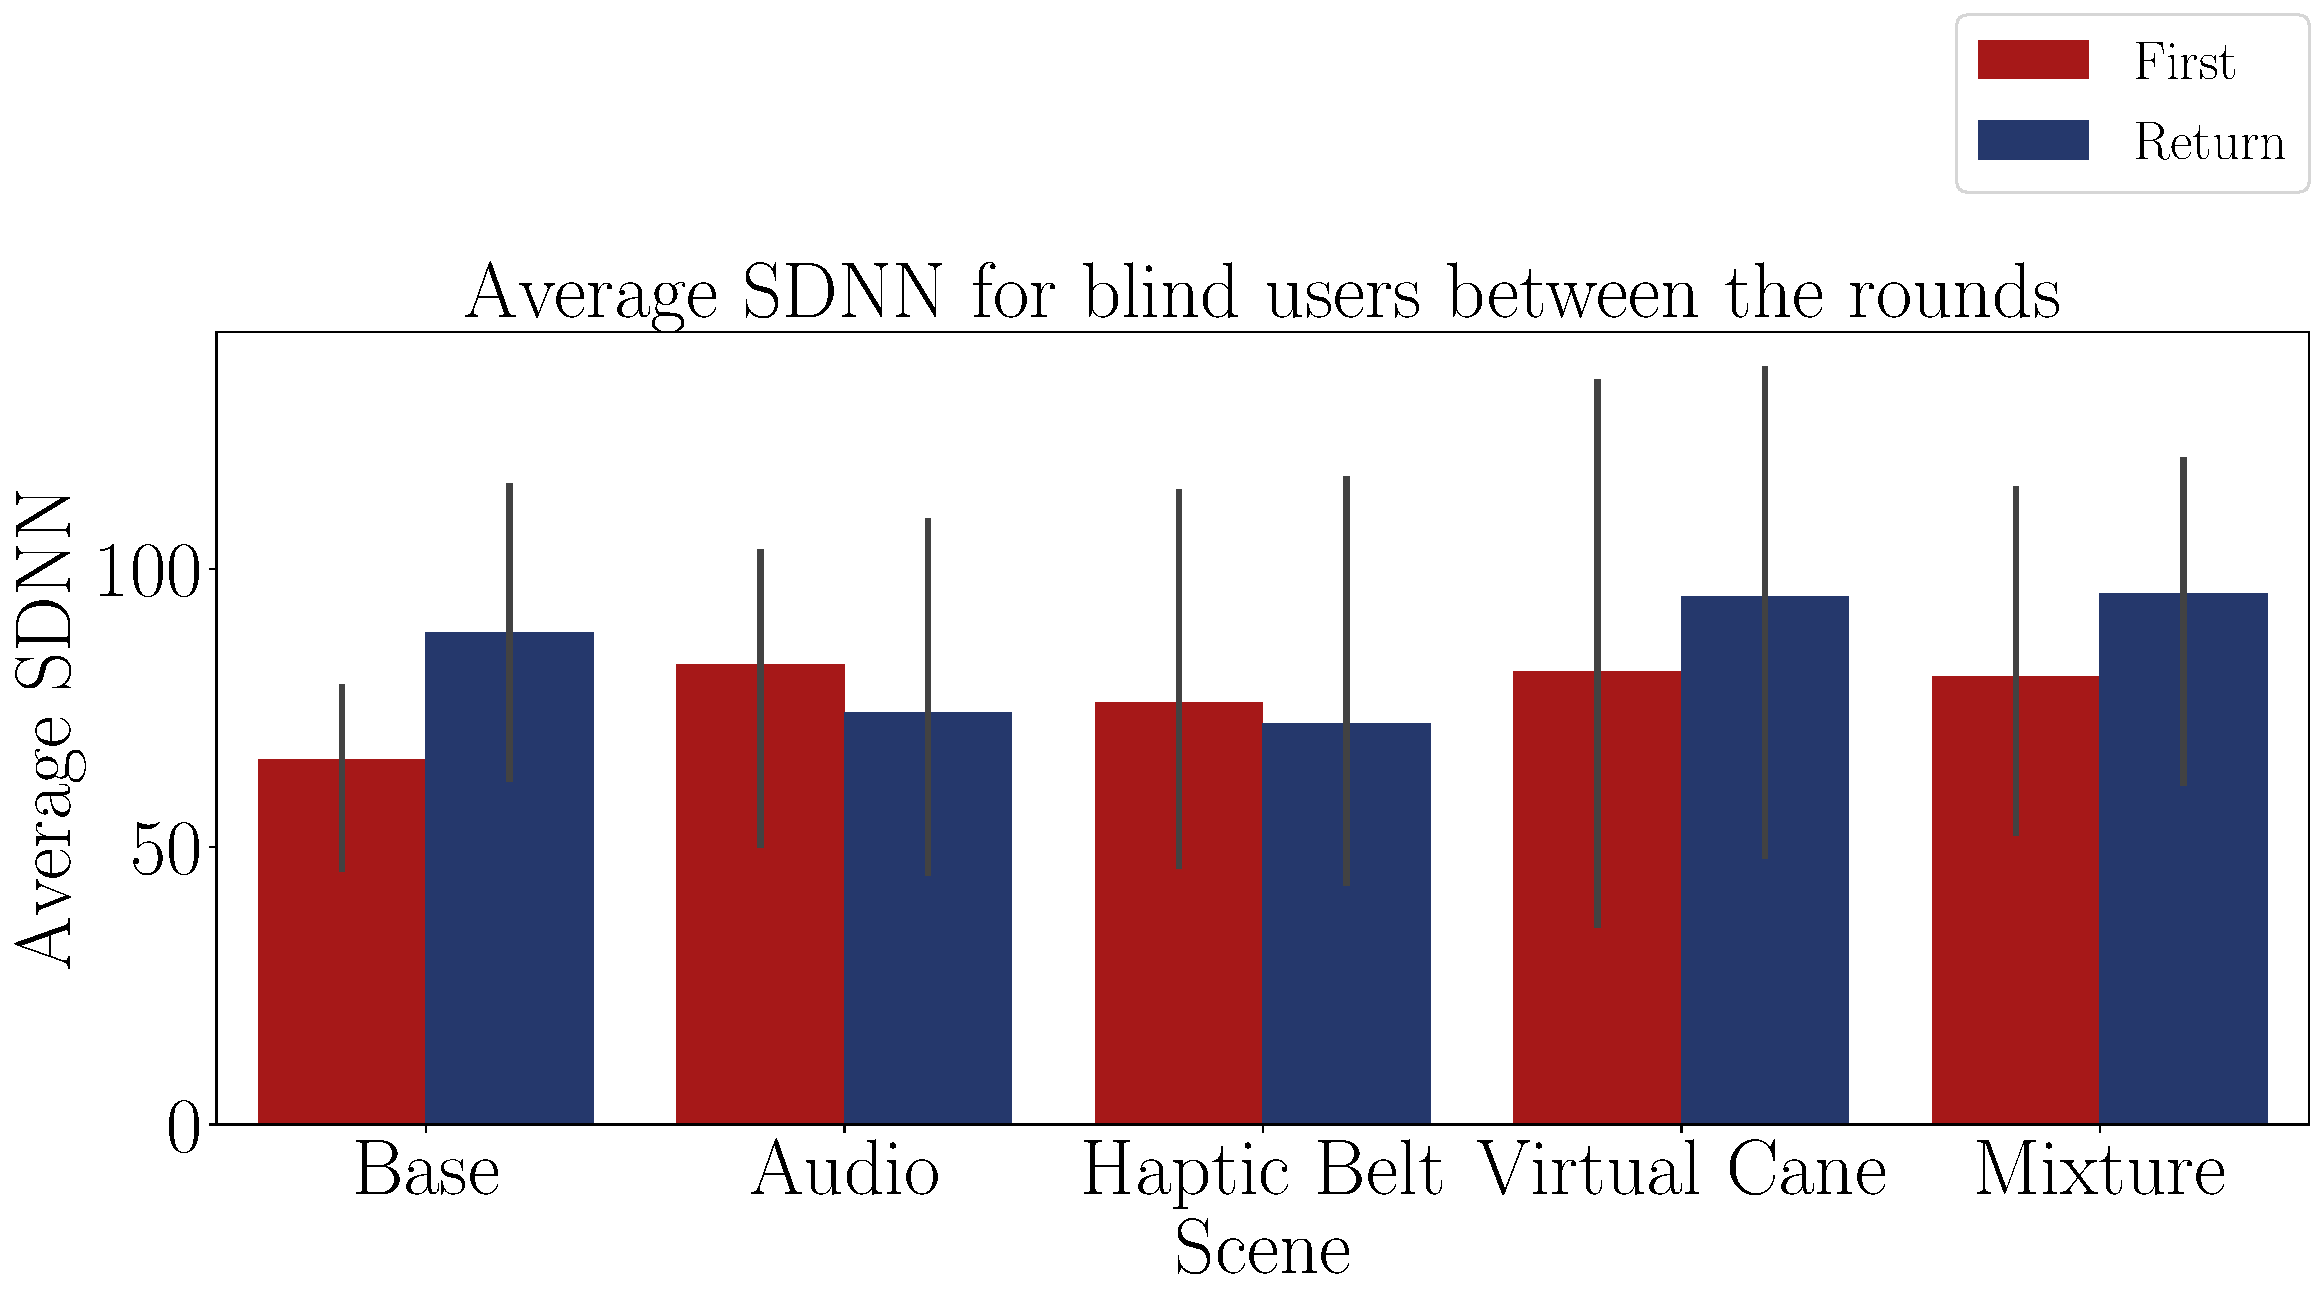
\includegraphics[width = 0.8\linewidth]{Resultados/ECG/Figuras/pdf/barplot_ecg_sdnn_5_scene_blind.pdf}
    \caption{Barplot of the average SDNN of the blind participants on each method.}
    \label{fig:barplot_ecg_sdnn_5_scene_blind}
\end{figure}

%The Table \ref{tab:sdnn_average_group_blind} presents the average SDNN variation between the rounds. It shows that only the "Audio" and the "Haptic Belt" methods shown a increase in the mental workload.
%
%
\begin{table}[!htb]
\centering
\caption{ECG average SDNN for each method of the blind participants.}
\label{tab:sdnn_average_group_blind}
\begin{tabular}{lrrrrr}
\toprule
{} &   Base &  Audio & Haptic Belt & Virtual Cane & Mixture \\
Visual Condition &        &        &             &              &         \\
\midrule
Blind            &  77.13 &  78.46 &       74.03 &        88.32 &   88.13 \\
\bottomrule
\end{tabular}
\end{table}



Figure \ref{fig:boxplot_ecg_sdnn_blind_scene} and Figure \ref{fig:boxplot_ecg_sdnn_blind_rounds} bring the SDNN barplot grouped by method and round. Apparently, there is a small tendency among the participants to increase the heartbeat in the ‘return’ round.

\begin{figure}[!htb]
    \centering
    \begin{minipage}{0.45\textwidth}
        \centering
        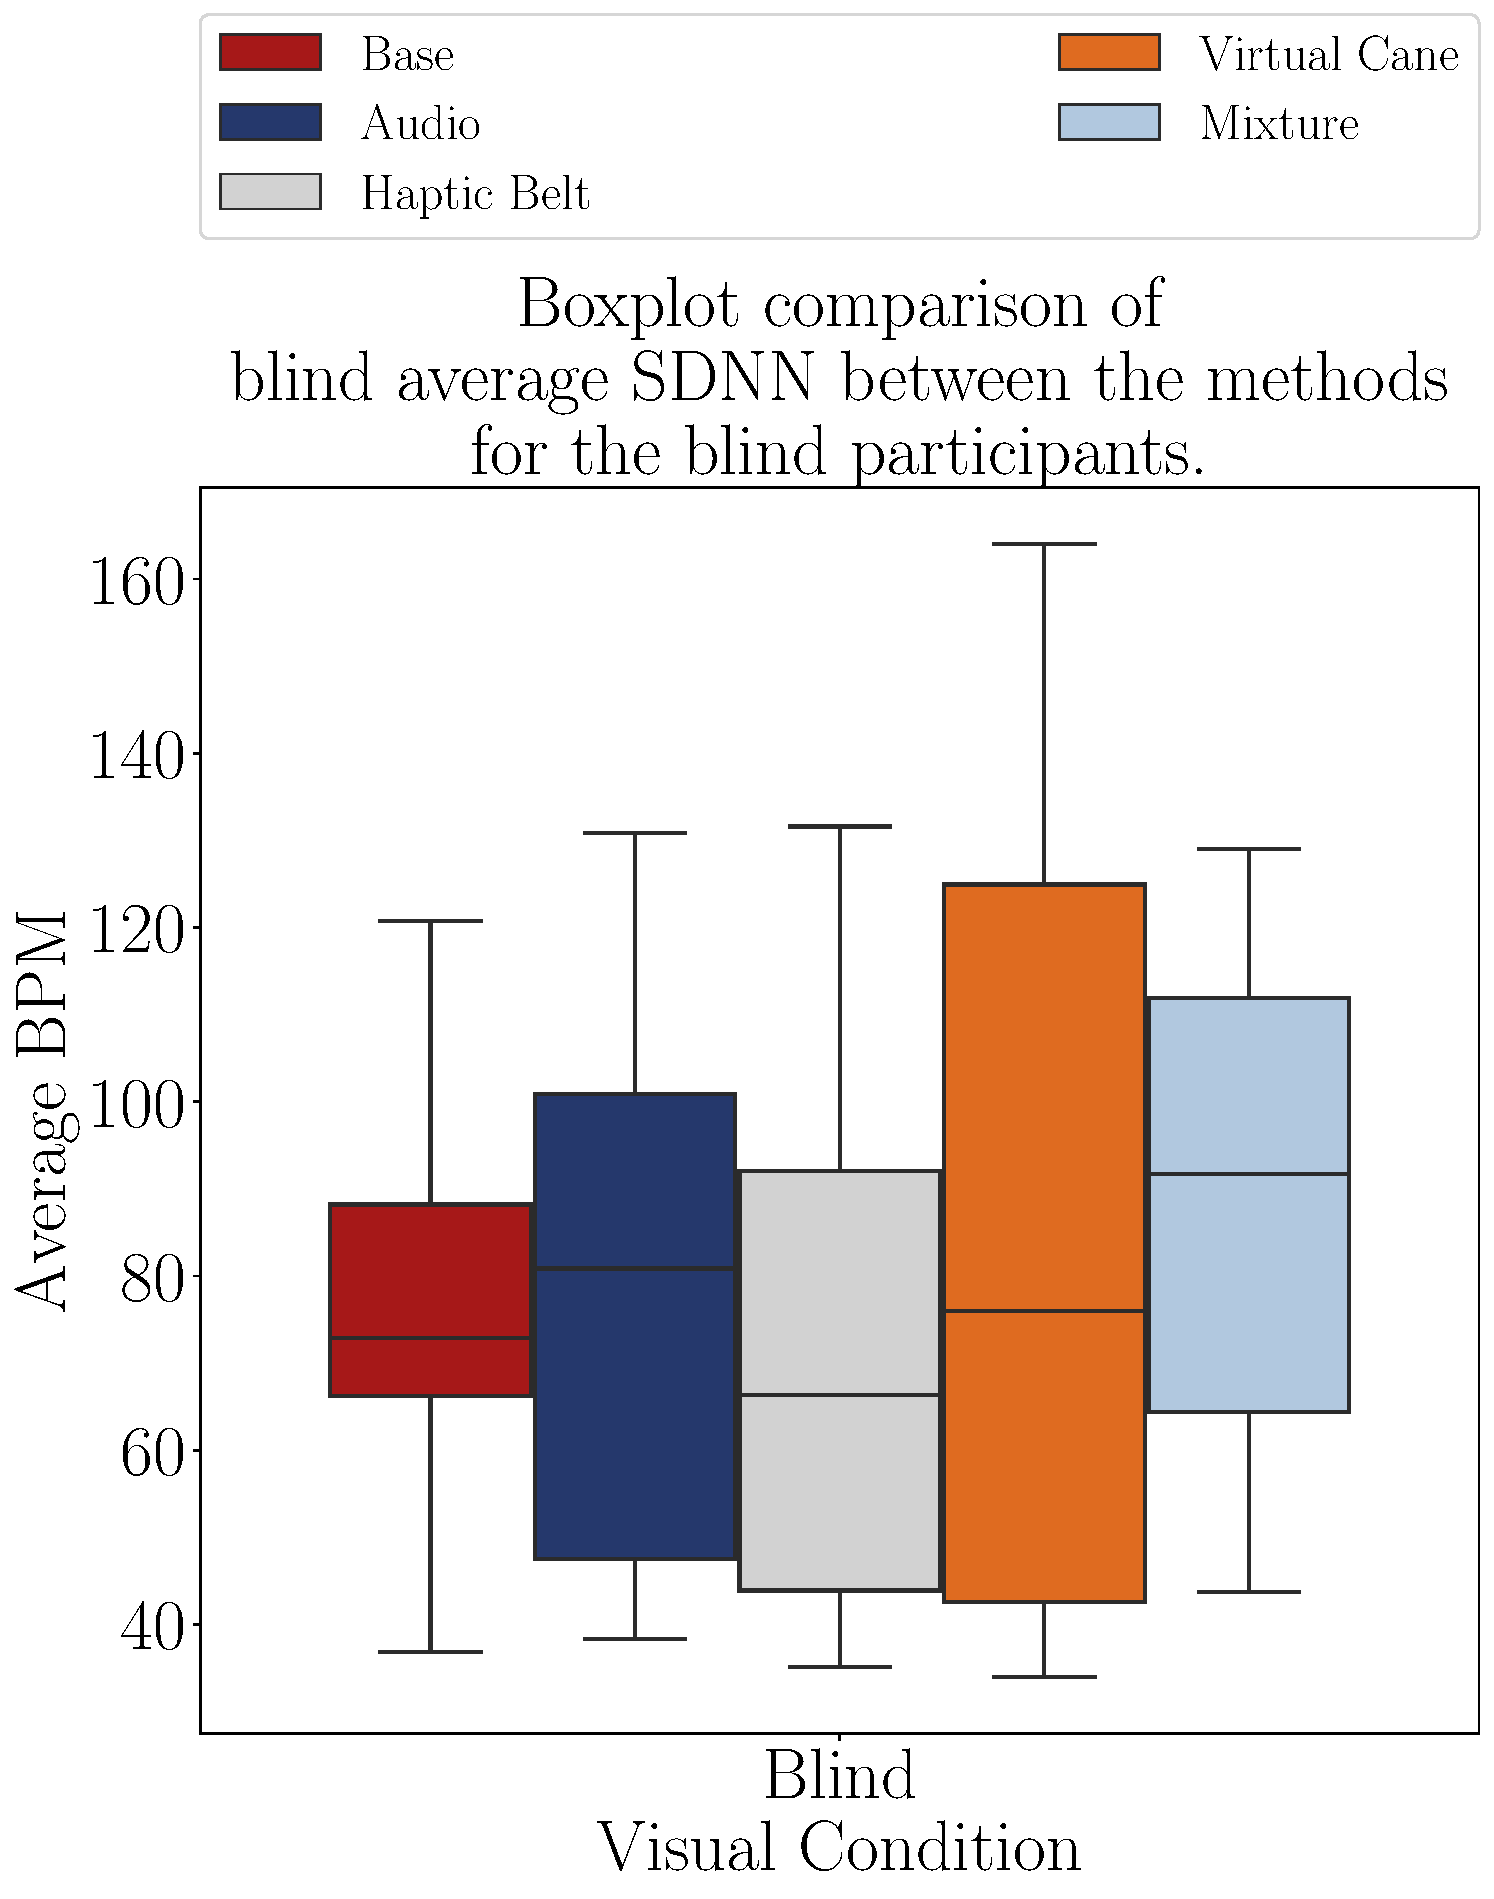
\includegraphics[width = 0.8\linewidth]{Resultados/ECG/Figuras/pdf/boxplot_ecg_sdnn_blind_scene.pdf}
        \caption{Boxplot of the SDNN of the blind participants grouped by method.}
        \label{fig:boxplot_ecg_sdnn_blind_scene}
    \end{minipage}
    \begin{minipage}{0.075\textwidth}
        \hfill
    \end{minipage}
    \begin{minipage}{0.45\textwidth}
        \centering
        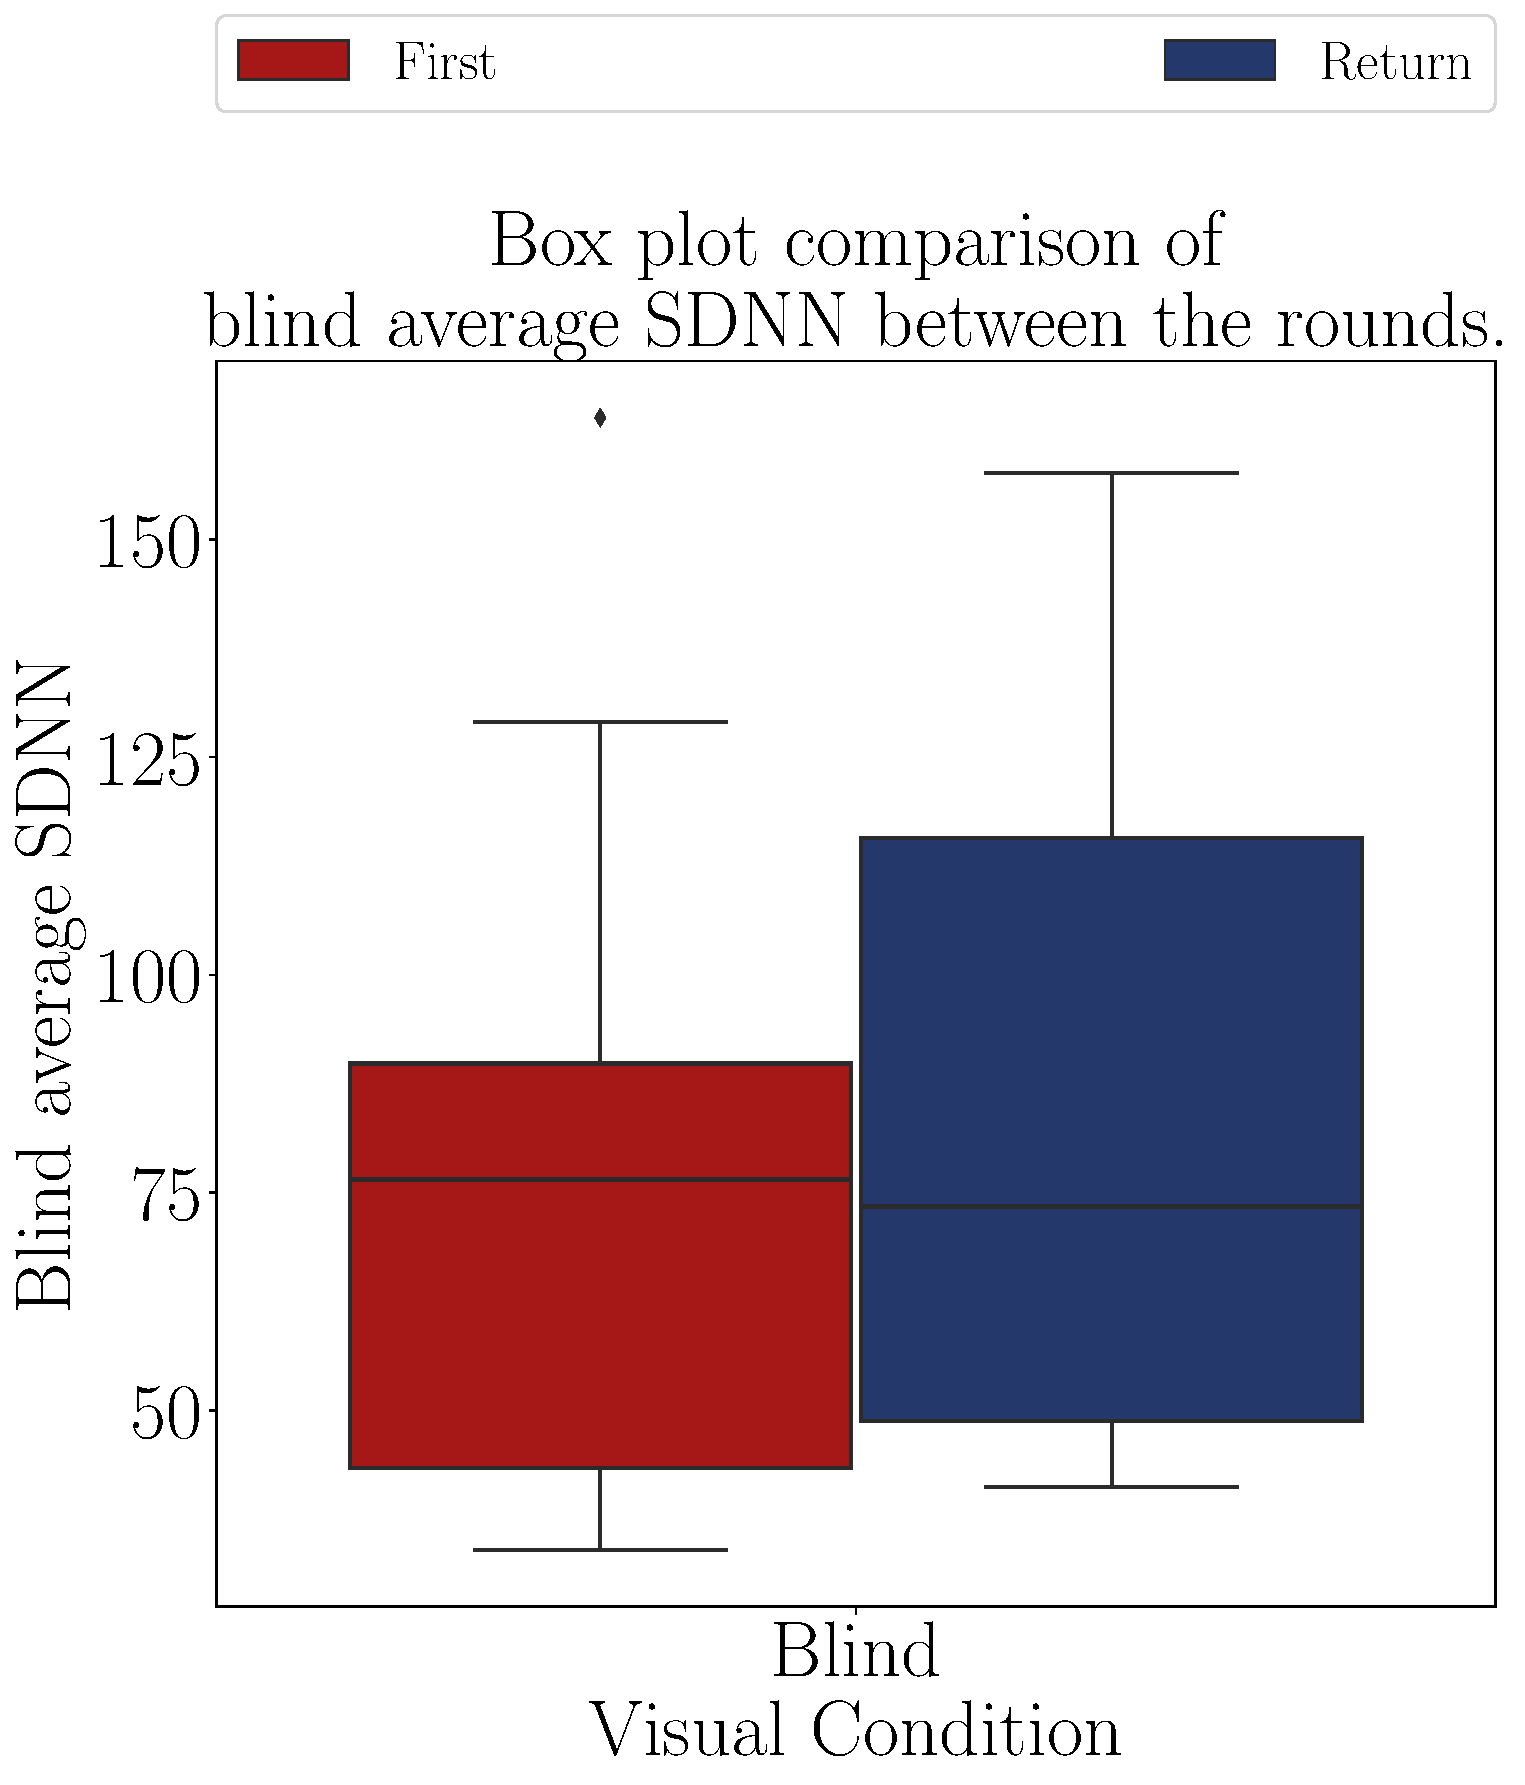
\includegraphics[width = 0.8\linewidth]{Resultados/ECG/Figuras/pdf/boxplot_ecg_sdnn_blind_rounds.pdf}
        \caption{Boxplot of the SDNN of the blind participants grouped by round.}
        \label{fig:boxplot_ecg_sdnn_blind_rounds}
    \end{minipage}
\end{figure}


Figures \ref{fig:qqplot_sdnn_two_way_blind} and \ref{fig:residplot_sdnn_two_way_blind} bring the QQ Plot and residual distribution. In this case, the residual distribution is more uniform than in Figure \ref{fig:residplot_bpm_two_way_blind}. The ANOVA results are presented in Table \ref{tab:blocdanova_sdnn_two_way_blind} and does not confirm any influence of the method or the round in the ECG heart rate variance.

\begin{figure}[!htb]
    \centering
    \begin{minipage}{0.45\textwidth}
        \centering
        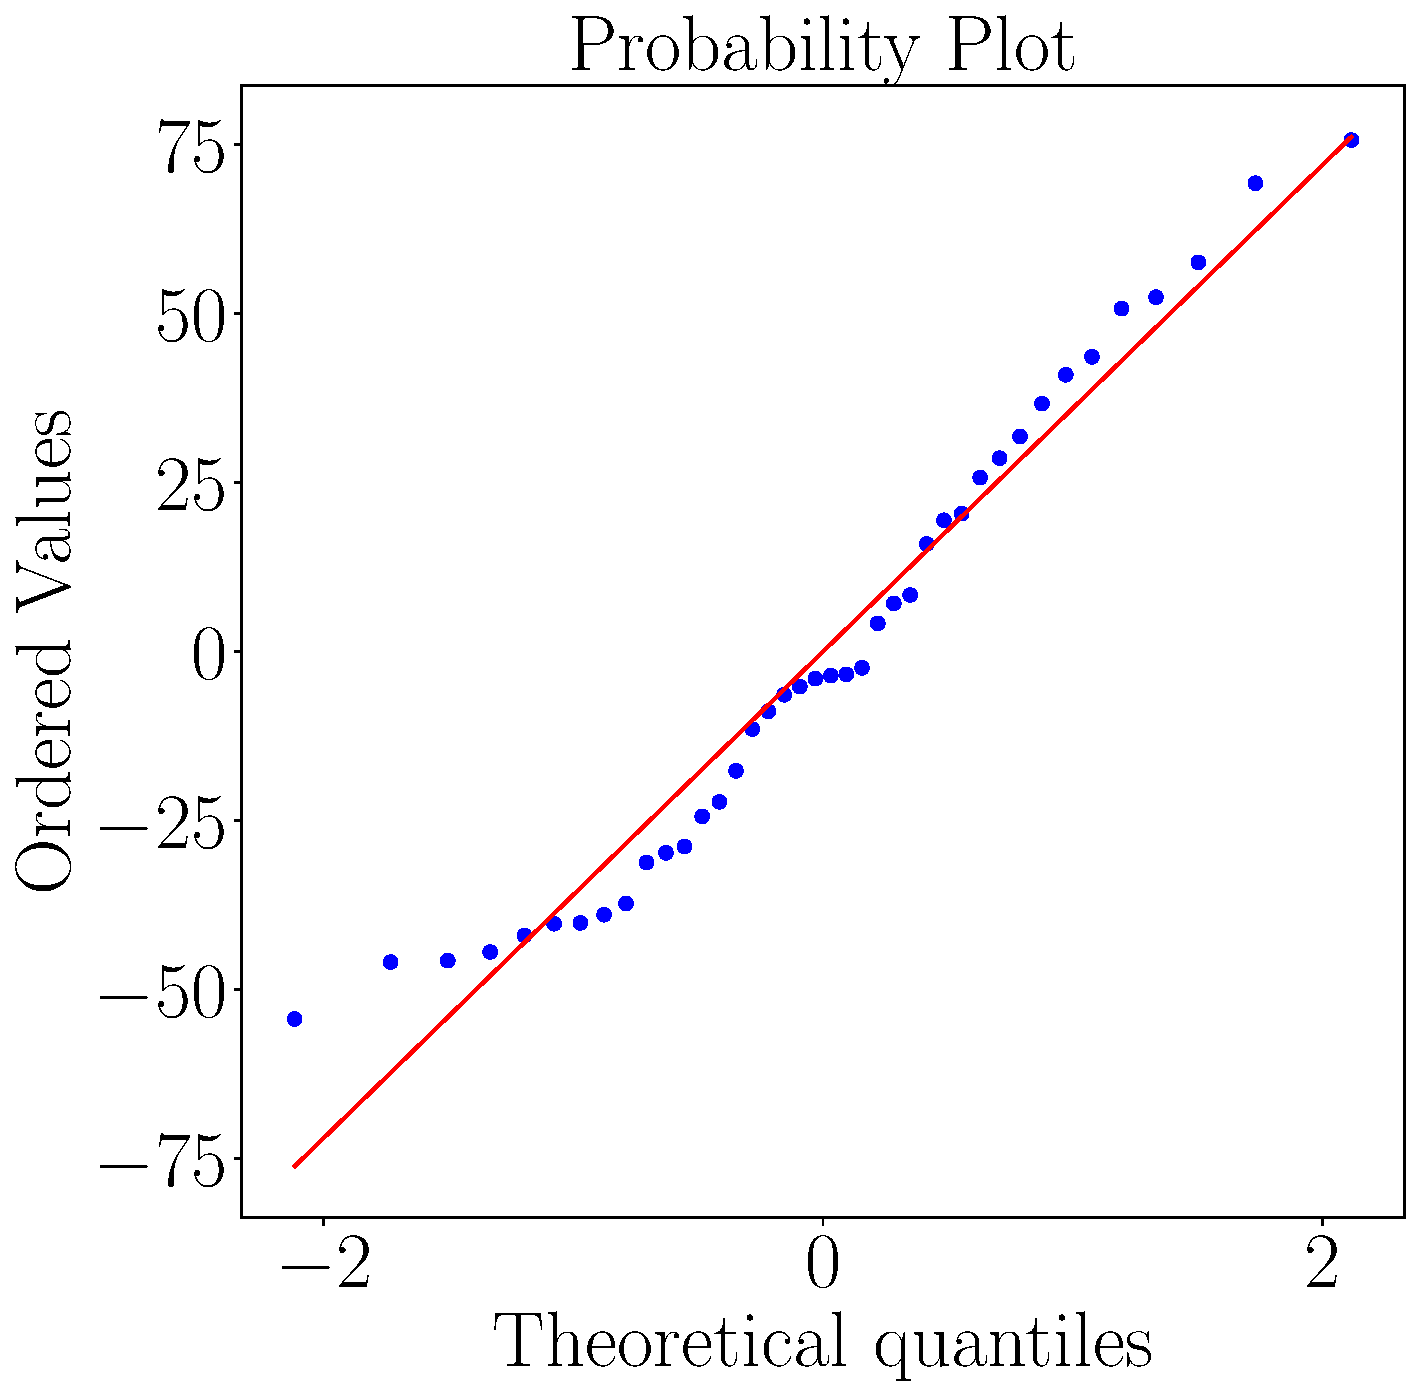
\includegraphics[width = 0.8\linewidth]{Resultados/ECG/Figuras/pdf/qqplot_sdnn_two_way_blind.pdf}
        \caption{QQ plot of the SDNN of the blind participants on each method.}
        \label{fig:qqplot_sdnn_two_way_blind}
    \end{minipage}
    \begin{minipage}{0.075\textwidth}
        \hfill
    \end{minipage}
    \begin{minipage}{0.45\textwidth}
        \centering
        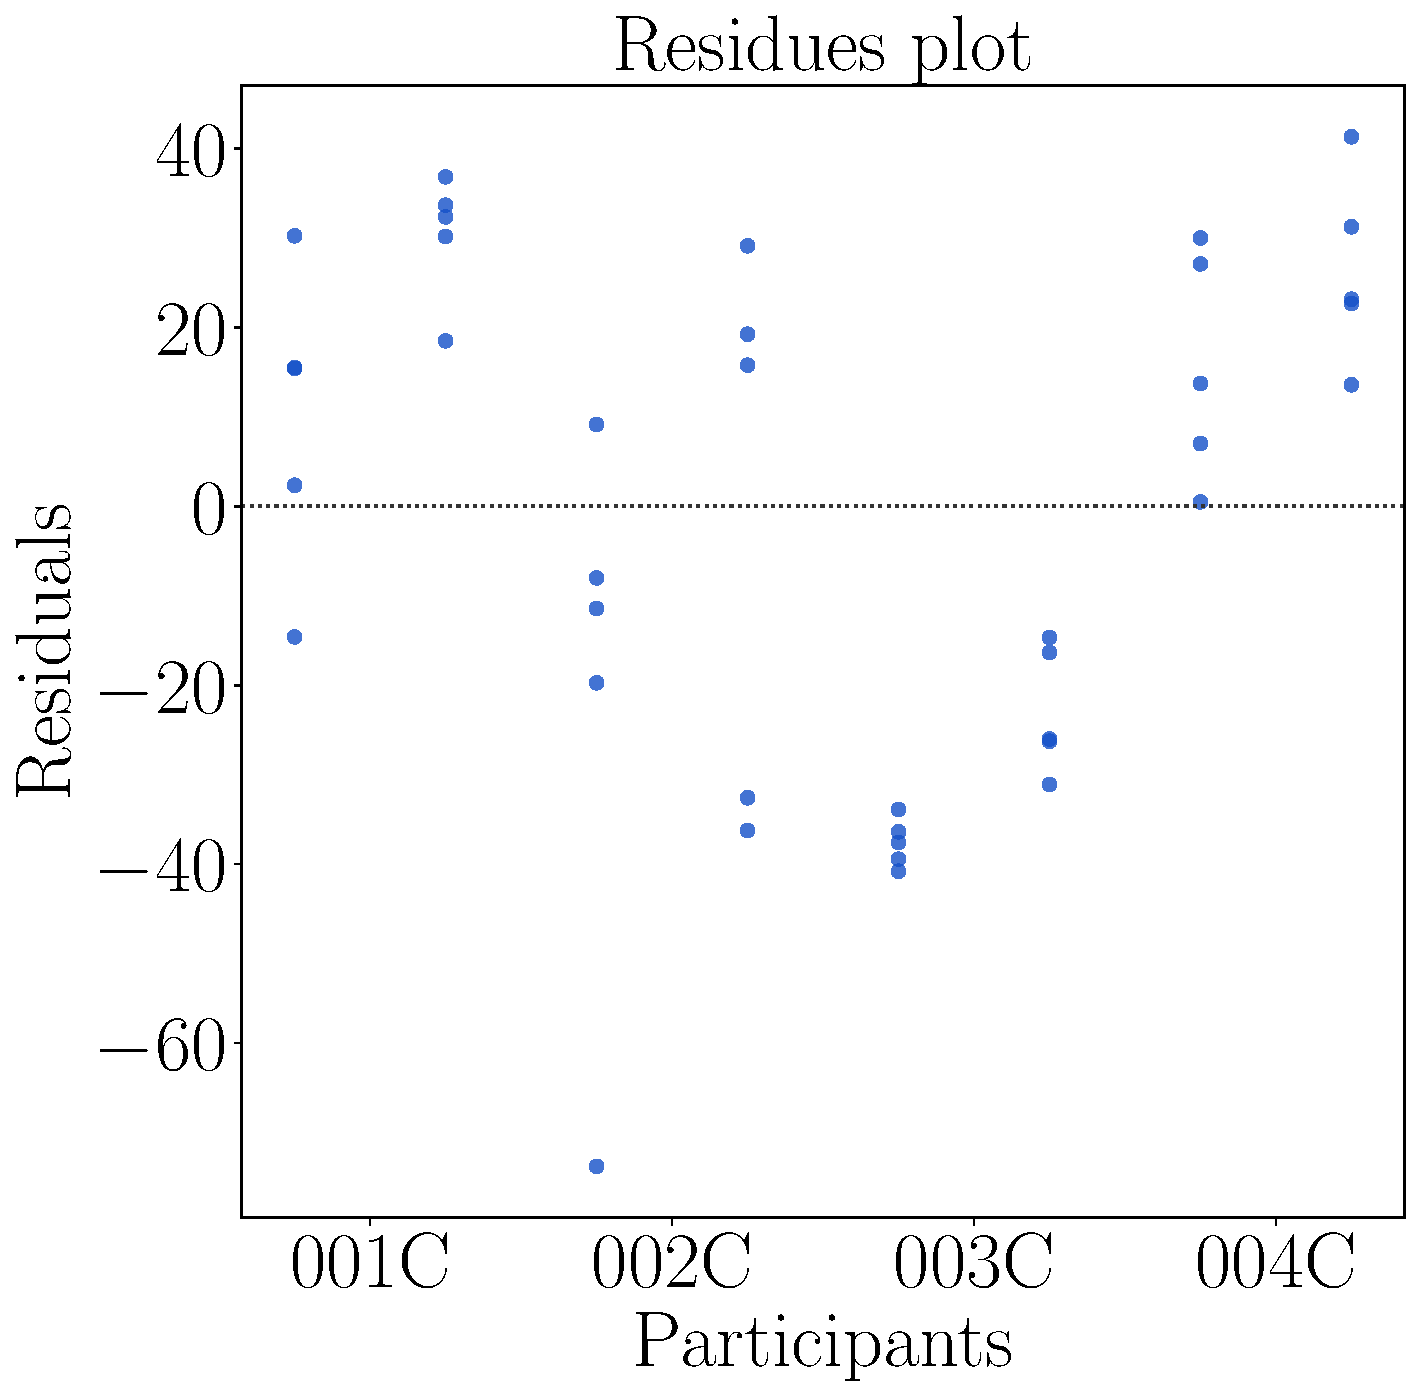
\includegraphics[width = 0.8\linewidth]{Resultados/ECG/Figuras/pdf/residplot_sdnn_two_way_blind.pdf}
        \caption{Residual plot of the SDNN of the blind participants on each method.}
        \label{fig:residplot_sdnn_two_way_blind}
    \end{minipage}
\end{figure}


\begin{table}[!htb]
\centering
\caption{Anova p-value for the average SDNN on each method for blinded users.}
\label{tab:blocdanova_sdnn_two_way_blind}
\begin{tabular}{lrrrrr}
\toprule
          Source & P-Value \\
\midrule
    \    Methods &   0.486 \\
     \    Rounds &   0.223 \\
\    Interaction &   0.473 \\
\bottomrule
\end{tabular}
\end{table}



\FloatBarrier